\section{Deployment of the application}\label{deployment}
The purpose of the web application is to allow multiple users to use the allocation application. To achieve this goal the web application needs to be accessible over the internet. To access the application over the internet it needs to be running on a computer with an associated url address, both a virtual computer and a url were provided by SDU to be used in this project. In this section I will discuss both the hosting of a web application and the flow from coding to deployment.\\
\begin{figure}[b!]
\centering
\hrule
\vspace*{0.2cm}
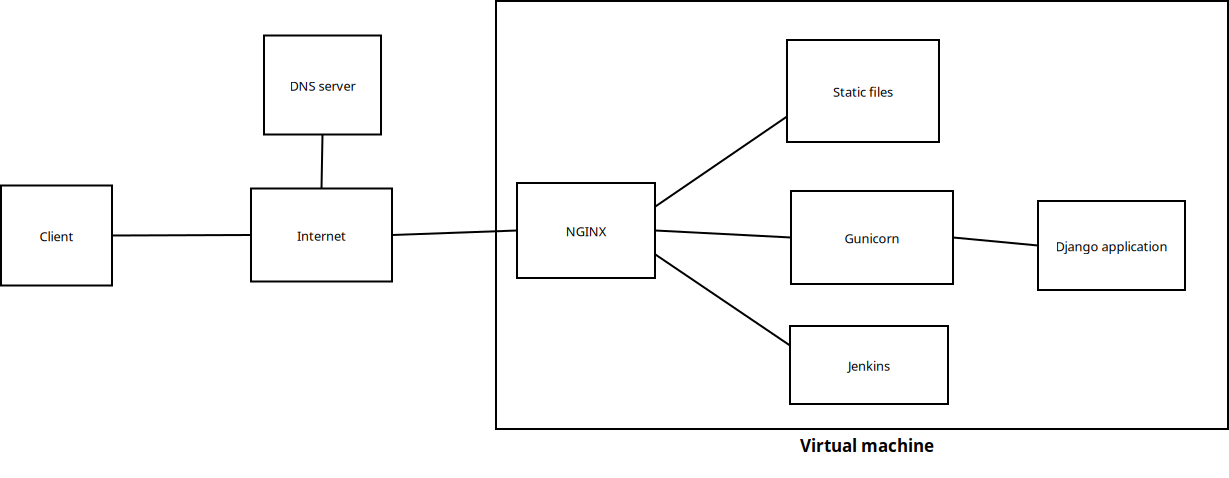
\includegraphics[width=\textwidth]{web_diagram}
\caption{Diagram illustrating the connections from client to application. \emph{NGINX} handles all requests arriving at the \emph{Virtual machine}. If the \emph{client} requests the \emph{Django application}, \emph{Gunicorn} responds with the templates from the \emph{Django application} while \emph{NGINX} responds with the \emph{Static files}. }
\label{fig:web_dia}
\end{figure}
\subsection{Hosting a web application}\label{sec:host}
When a client wants to visit the application, they navigate to the url address of the application in their web browser, a DNS request is then send to a DNS server to match the url with the IP address of the server on which the application is running. The clients web browser then sends a request to the server, requesting to view the application. The incoming request is then routed to the application which responds with the requested page. The connections established in this flow is illustrated in figure \ref{fig:web_dia}.\\\\
On the virtual machine an instance of NGINX is running as a reverse proxy which forwards all incoming requests to the requested application and serves static files like images, javascript and css files. Typically requests for websites are send to port 80 for http, and port 443 for https.\\\\The running instance of NGINX is configured to redirect any incoming requests on port 80 to port 443 in order to ensure all traffic is encrypted using TLS\footnote{Many online resources use SSL/TLS when referring to this encryption, the last version of SSL was however \href{https://datatracker.ietf.org/doc/html/rfc7568}{deprecated in 2015} which is why I will refer to it only as TLS}.\\\\
TLS is a combination of asymmetric and symmetric encryption used to encrypt communication over the internet. To use TLS the server needs a certificate along with a public/private key pair\cite{encrypt}.\\
When an https request reaches the server, the server responds with its certificate and public key. The client then verifies that the certificate is legitimate by asking a trusted certificate authority if the certificate is valid to ensure that the communication is between it and the expected server.\\
When the certificate has been verified the server and client communicates to each other what types of encryption they support, in order to use the strongest available. The client then uses the servers public key to encrypt a session key to be used for the current session and sends it to the server, which uses its private key to decrypt the session key. From that point and until the connection is closed, all requests and responses are encrypted using symmetric encryption.\\\\
In the case of this project a self signed certificate was used. A self signed certificate means the server can not be verified by an outside authority since anyone could have signed it. However the provided virtual machine itself sits behind a reverse proxy managed by SDU which handles the encryption of traffic to the internet and by extension the actual certificate used when accessing the application.
%To generate a private/public key pair and a certificate on the server the application openssl was used. In a setting where traffic to the server would come directly from the internet without involving SDU, the certificate created by openssl would need to be signed by a certificate authority in order to verify its authenticity, alternatively Let's Encrypt can be used to obtain a signed certificate. A signed certificate does not last forever and has to be renewed at certain intervals, this can be automated with a tool like Certbot which obtains a certificate from Let's Encrypt and renews it every 60 days.
\begin{figure}[b]
\centering
\hrule
\vspace*{0.2cm}
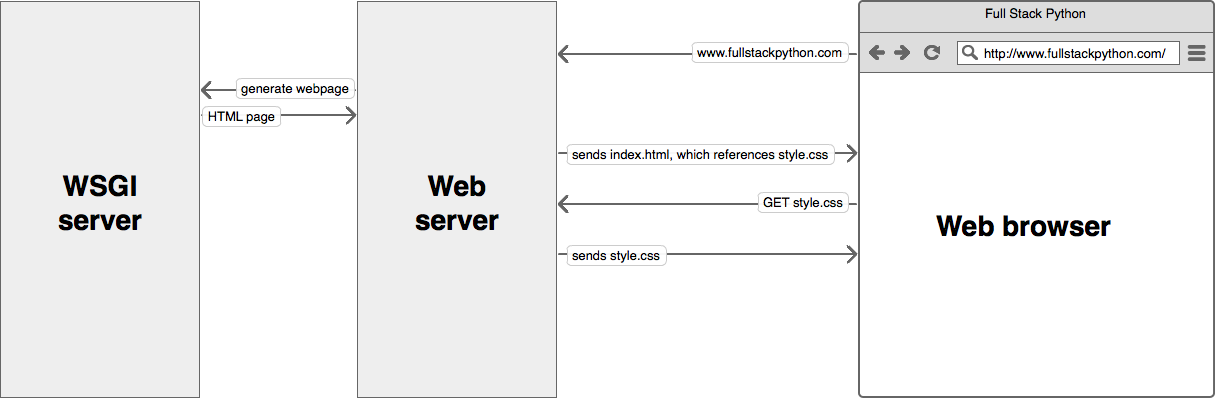
\includegraphics[width=\textwidth]{web-browser-server-wsgi}
\caption{Diagram from \href{https://www.fullstackpython.com/wsgi-servers.html}{Full stack Python} illustrating the requests and responses between client, Web server(NGINX) and WSGI server(Gunicorn)}
\label{fig:baf}
\end{figure}
\\\\
As illustrated in figure \ref{fig:web_dia} the running instance of NGINX handles traffic to and from three resources: The Django application, an instance of Jenkins which will be discussed in the next section and the static files used by these applications. Since the Django application itself is just a collection of python scripts which is not runnable by a traditional web server, a web server gateway interface(WSGI) is needed to run the python application. Django does set up a minimal WSGI configuration when a new project is started and includes a lightweight development server which according to the \href{https://docs.djangoproject.com/en/4.2/ref/django-admin/#runserver}{documentation} should only be used in a development environment. I chose to use Green Unicorn(Gunicorn) as the WSGI server for this particular project.\\
When a request from a client is send to Gunicorn its job is to handle that request and respond with an html page, the page may contain images and styling defined in a css file which is then served by NGINX, illustrated in figure \ref{fig:baf}.


\subsection{From development to production} \label{sec:dev_to_prod}
During the development of the application i used git as version control system to store the code and keep track of changes. Early in the development of the web application, it became apparent that manually accessing the virtual machine on which the application is hosted via ssh and then downloading the most recent version from git to update the version being hosted on the server, was a time consuming and inefficient way of updating the application. And that I needed a way to automate this process, the solution was to use a CI/CD tool\cite{redhat_cicd}.
\begin{figure}[b]
\centering
\hrule
\vspace*{0.2cm}
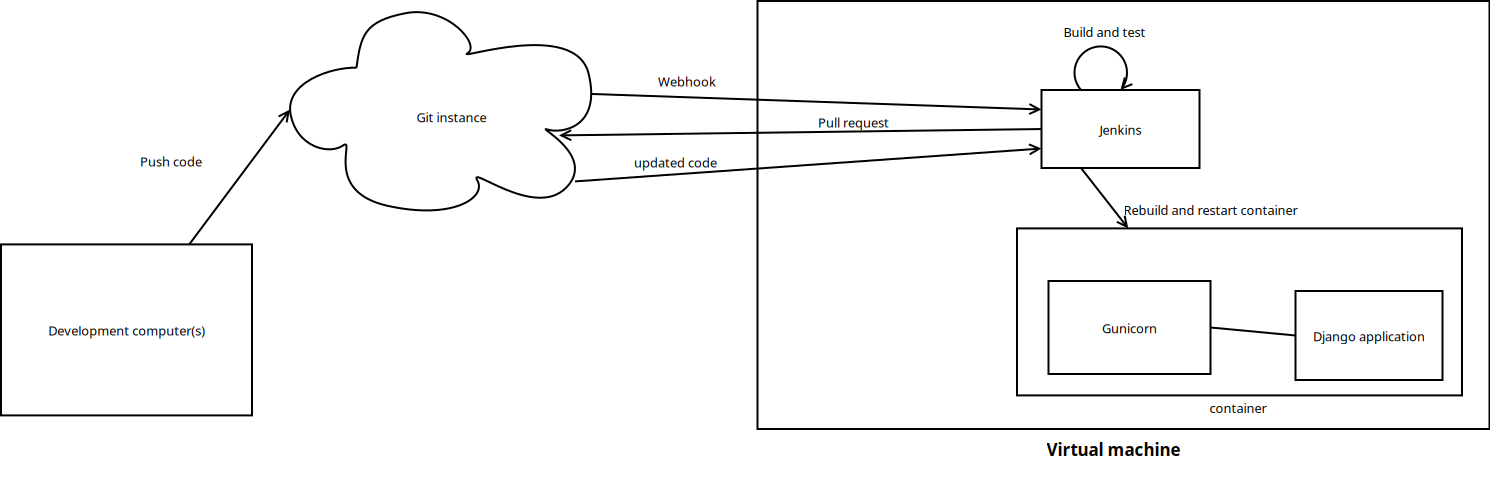
\includegraphics[width=\textwidth]{pipeline_dia}
\caption{Diagram illustrating the flow from code to running application through git and Jenkins}
\label{fig:pipe}
\end{figure}
\\\\
Many different tools exists in this space so to limit the potential candidates I came up with a list of requirements the tool had to fulfil:
\begin{enumerate}
	\item It had to be free of charge.\\At the very least there had to be a free version I, as a student, could use for this project.
	\item It had to run on the virtual machine.\\Since access to the machine was limited to connections originating from SDU's network the tool should run on the computer that hosted the application.
	\item It had to support python.
	\item It had to be able to build and deploy Docker containers, more on this in section \ref{sec:cont}.
\end{enumerate}
The first two requirements in particular limited the number of potential candidates and in the end I decided to use Jenkins since it fulfilled all the requirements.\\
Jenkins has very good documentation and easy to follow guides, while still being a very powerful tool with many advanced features which is extensible by a large library of plug-ins. It has a webUI in which all settings can be accessed, and a complete NGINX configuration is available on the Jenkins website\cite{jenkins_nginx} to allow access over the internet.\\\\
Setting up the steps needed to pull and deploy the updated code was fairly straight forward since i was able to run the commands previously used to update the running instance of the application, from within Jenkins.\\
With the inclusion of Jenkins the path from code to running application, also called the pipeline, executes the following steps as illustrated in figure \ref{fig:pipe}:
\begin{itemize}
	\item Manually push changes to the git repository.
	\item A git webhook sends a ``notification'' to Jenkins that a push has happened.
	\item Jenkins pulls the updated code from the repository.
	\item Jenkins builds and tests the updated application in a test environment.
	\item Assuming the building and the tests pass, Jenkins again builds the updated container this time in the live environment, and restarts the running instance of the application with the updated container.
\end{itemize}
If the tests does not pass or the building process fails the step that failed can be viewed in the webUI.
\subsubsection{Containerisation}\label{sec:cont}
The provided virtual machine runs linux as its operating system, I did not however want to limit the application to running on a specific operating system on which a user would have to install multiple specific programs and python packages in order to use the application. To run the application regardless of the operating system of the host machine, and to better control the environment in which the application would be running, containers provided the solution I needed.\\\\
Using Docker allows me to package all the individual components, NGINX, Jenkins and my web application along with Gunicorn, in separate containers each containing only what is needed to run an instance of the specific application and the only requirement for the host system is that it should be able to run Docker. It allows anyone to quickly start the applications and achieving an equivalent setup, by setting a few variables and then, with the use of Docker Compose, starting all containers with a single instruction given to Docker. All the instructions on how to build the individual containers are defined in a container specific dockerfile, this file defines which application or environment is needed and which operations should be performed in order to build the container. A Docker Compose file then defines what containers to start, the order in which they should be started and the networks and volumes available to the containers.\\\\
The variables that would need to be adjusted in order to start the applications on another machine are all contained within a \verb|.env| file located in the same folder as the Docker Compose file. This file contains settings for both the Docker containers and for the Django application. This approach means that all variables, like where to store static files and the secret keys used for authentication, can be changed in a single place. Since this file contains secret keys it should not be uploaded to the git repository and is therefore ignored when changes are being tracked by git. Instead this file is manually transferred to the virtual machine, used for hosting the application.